\documentclass{article}
\usepackage{import}
\subimport{../}{preamble}
\begin{document}

\section{AFM Design: Measurements of Force}

\begin{wrapfigure}{O}{0.38\textwidth}
\centering
\vspace{-10pt}
\fontsize{10pt}{1em}\selectfont
\def\svgwidth{\textwidth}
\subimport{./figures/}{figures/afm_concept.pdf_tex}
\caption[Concept of contact mode AFM]{\textbf{Concept of contact mode AFM.} An applied force $F$ bends the cantilever proportional to a linear displacement $x$. Light incident on the bent cantilever deflects at an angle $2\theta$.}
\label{fig:afm_concept}
\vspace{-5pt}
\end{wrapfigure}

% AFM concept
Force is measured using an atomic force microscopy (AFM) module to measure cantilever deflections as they flex under an applied force. The linear displacement of the cantilever, $\Delta z$, from its equilibrium position under an applied force, $F$, is given simply by,
\begin{equation} F=k\Delta z, \label{eq:hookes_law} \end{equation}
where $k$ is the stiffness or spring constant of the cantilever. Contact and tapping mode cantilevers are most used in experiments, for which $k=\SI{0.2}{\newton\per\metre}$ and \SI{40}{\newton\per\metre}, respectively. The change in angle caused by a linear displacement at the tip can be measured optically as a change in deflection angle of a laser focussed on the back of a reflective cantilever. This sensitivity of this technique has led to it being named atomic force microscopy since atomic-scale forces cause measurable deflections enabling topological imaging with {\color{red}atomic/sub-nm} resolution.
For tip-tip systems nano-scale force measurements become important as they dictate how tips come together and move through interfacial layers prior to electrical contact. To this extent a compact AFM module was constructed to monitor the tip-tip interaction forces during tip dimer {\color{red}measurements/experiments/scans}.

% AFM design
The AFM module consists of a compact optomechanical {\color{red}array} mechanically bolted onto the top plate of the microscope platform and a separate \SI{633}{nm} laser diode coupled together using strain-relieved single mode fibre. Single mode fibre is used to produce a stabilised laser output.%
\footnote{Stabilised output results from single mode operation. Multimode stability leads to significant intensity changes that cause issues with the lateral effect photodiode.}
Light is focused through an entry window in the experimental chamber onto the cantilever of the soft AFM probe in an experiment. The beam position is laterally offset on the focussing lens using a silver turning prism to focus on the cantilever at an angle so that reflections return through the AFM with the opposite lateral offset. An alternative to this approach allows use of a common beam path but requires two polarisers and a quarter wave plate, leading to simpler alignment but a more costly design. As the light is reflected back off the cantilever at a different angle in the focal plane it is laterally translated in Fourier space. This translation is measured using a fast lateral effect photodiode, also known as a position sensitive detector (PSD). The PSD contains a signal processing circuit with an in-built transimpedance amplifier to convert the small currents into voltages corresponding to the measurements $\Delta x,y$ and $\sum x,y$. Voltages are recorded using a DAQ card (NI X-series). A diagram of this arrangement is shown in \figurename~\ref{fig:afm_design}.

\begin{figure}[bt]
\centering
{\fontsize{9.5pt}{1em}\selectfont
\def\svgwidth{0.8\textwidth}
\subimport{./figures/}{figures/afm_schematic.pdf_tex}}
%\includegraphics[width=0.8\textwidth]{figures/afm_schematic}
\caption[Schematic diagram of the AFM module.]{\textbf{Schematic diagram of the AFM module attached to the side of the microscope platform.} Incident light from a single mode fibre is focussed at an angle onto an AFM cantilever. Angled reflections from the cantilever are re-collimated into a laterally displaced beam whose position is detected on the PSD.}
\label{fig:afm_design}
\end{figure}

% Limitations to beam size and focal lengths
The width of the cantilevers used and the radius of the input beam determines the minimum beam size. The cantilevers have a width of \SI{50}{\micro\metre} and therefore the spot size in the focus must be less than this value. Since the input is a single mode Gaussian beam the spot diameter, $2w_0$, can be calculated using,
\begin{equation} 2w_0 = \frac{4\lambda}{\pi}\frac{f}{D}, \end{equation}
where $f$ is the focal length and $D$ is the collimated beam diameter %\cite{Newport}. %http://www.newport.com/Gaussian-Beam-Optics/144899/1033/content.aspx
For $\lambda=\SI{633}{nm}$ and a required spot size $2w_0 < \SI{50}{\micro\metre}$ the fraction $f/D < 62$. The focal length is optimised first as there is a limit imposed by the distance from the edge of the top plate to the objective focus through the chamber window. For this reason a \SI{100}{mm} lens is chosen, which restricts the beam diameter to $D > \SI{1.6}{mm}$. The beam diameter is set by the short focal length lens collimated the single mode fibre output and the iris afterwards.

% Determining position from current or voltage
Changes in the voltage output of the PSD are correlated with force applied to the tip at the end of the cantilever allowing the applied force to be measured. The position of the PSD is adjusted with zero force applied to an AFM cantilever so that zero voltage corresponds to zero applied force. The lateral displacement of the returning beam is then calculated using,
\begin{equation}
ds_{x,y} = \frac{\Delta V_{x,y}}{\sum V_{x,y}},
\end{equation}
where $i$ is the lateral axis, either $x$ or $y$.

\subsection{Calibrating the AFM}

The displacement of the tip under an applied force can be related to the translation of the beam as a measured voltage. By determining the displacement the force applied to the AFM tip can be measured using \eqref{eq:hookes_law}. The transformation from displacement into a measured voltage signal can be expressed as,
\begin{equation}
V = k_{x \rightarrow V}x,
\end{equation}
where $k_{x \rightarrow V}$ is the transformation. In the current geometry this transformation is linear and therefore $k_{x \rightarrow V}$ is a fixed constant $k_{x \rightarrow V}$ for a given AFM beam alignment. In general $k_{x \rightarrow V}$ includes each of the transformations required to convert the cantilever displacement into a measurable signal. These transformations are apparent when following the path of the laser beam through the AFM module. The displacement needs to be converted into an angular cantilever deflection, which is further transformed into a translation of the beam after the lens-induced Fourier transform. At this point the displacement requires converting into a current on the PSD and then to the measured voltage after amplification by the \num{e5} gain transimpedance amplifier in the signal processing circuit. Each of these is a linear operation hence the overall effect can be expressed in a single constant $k_{x \rightarrow V}$, which can be experimentally determined.

The simplest method of calibration involves pushing an AFM tip against a hard contact so that the displacement is known ($\Delta z = z$). From there the voltage is measured as a function of displacement and data can be fitted to determine $k_{x \rightarrow V}$. The force can then be estimated using \eqref{eq:hookes_law}. Whilst this is not ideal as the cantilever spring constant is still somewhat unknown, the method is simple. Therefore, for force measurements, the value of the cantilever spring constant $k$ from the AFM probe data sheet is assumed. The large tolerances on stiffness measurements are not ideal and mean that this approach is only sufficient to estimate the applied force on a nano-gap to within {\color{red}less than an order of magnitude}% calculate an actual value based on percentage error
. Other methods of accurately measuring the cantilever spring constant do exist, as do methods to directly map the force to a measured signal, i.e., $F = k_{V \rightarrow F}V$ \cite{hutter1993calibration, senden1994experimental, torii1996method, sader1999calibration, levy2002measuring, cumpson2004quantitative, gates2007precise, langlois2007spring, ohler2007cantilever}, but add further {\color{red}complexity/complications/requirements} to experiments. Since exact measurements of force are not crucial to current nano-gap studies, less than an order of magnitude is an acceptable uncertainty.

\FloatBarrier
\end{document}